\documentclass[paper = a4]{scrartcl}

\usepackage[T1]{fontenc}
\usepackage[utf8]{inputenc}
\usepackage[ngerman]{babel}
\usepackage[autostyle = true, german = quotes]{csquotes} % Anführungszeichen

\usepackage{amsmath}
\usepackage{graphicx}

\begin{document}

\subject{Praktikum Multicore"=Programmierung}
\title{Protokoll zu Projekt~6: Mehrgittermethoden}
\author{Florian Klemme \and Manuel Leßmann}
\maketitle

\section{Jakobi- und Gauß-Seidel-Verfahren}

\begin{quote}
    a) Programmieren Sie eine serielle Version des Jakobi"=Verfahrens. Gegeben sei dazu [\dots] \(f(x, y) = 32(x(1 - x) + y(1 - y))\). Beachten Sie dabei auch die Randbedingungen [\(u(x, y) = 0 \quad \forall (x, y) \in \Gamma\)]. Verwenden Sie zur Überprüfung Ihres Programms auf Korrektheit die analytische Lösung \(u(x, y) = 16x(1 - x)y(1 - y) \quad \forall (x, y) \in \Omega\).
\end{quote}

Gemacht. Implementierung scheint auch korrekt zu sein, da nur eine minimale Abweichung zur analytischen Lösung besteht. Ansonsten gibt's hier nichts zu zeigen/schreiben. Kann wohl am Ende hier im Protokoll entfallen.

\begin{quote}
    b) Implementieren Sie ebenfalls eine serielle Version des Gauß"=Seidel"=Verfahrens. Vergleichen Sie die gewonnenen Ergebnisse mit den Ergebnissen des Jakobi"=Verfahrens. Was fällt beim Vergleich der Iterationsschrittzahlen sowie der Laufzeiten beider Verfahren über verschiedenen Verfeinerungen (\(h = \frac{1}{2^l} \text{ mit } l = 1, 2, \dots, 6, \dots\)) auf?
\end{quote}

Der Unterschied zu Jakobi in der (sequenziellen) Implementierung ist marginal, daher habe ich sie kurzerhand hinzugefügt. Messungen habe ich noch keine angestellt.

Hier ist bestimmt \(h = \frac{1}{2^{l} + 1}\) gemeint. Zumindest macht diese Unterteilung später im Mehrgitter"=Verfahren Sinn, da \(h = \frac{1}{2}\) \emph{linker Rand -- Punkt -- rechter Rand} bedeutet, also ein Grid mit nur einem Punkt. (ungerade, schlecht halbierbar)

\begin{quote}
    c) Messen Sie mit Hilfe der in a) angegebenen analytischen Lösung für beide Verfahren den maximalen Approximationsfehler mit Hilfe der euklidischen Norm in jedem Iterationsschritt und für ein gewähltes h und stellen Sie diesen graphisch dar.
\end{quote}

Euklidische Norm bedeutet hier wohl: einfacher Abstand. Noch nicht implementiert.

\begin{quote}
    d) Da hier innerhalb eines einzelnen Iterationsschritts keine Datenabhängigkeiten zu finden sind, lässt sich das Jakobi"=Verfahren durch einfaches Aufteilen der Berechnungen auf verscheidene Prozessoren und Kommunizieren eventueller Überlappungen parallelisieren. Entwerfen Sie eine parallele Version des Verfahrens (wahlweise mit OpenMP oder Cuda/OpenCL) und verifizieren Sie Ihre Ergebnisse gegenüber der seriellen Variante.
\end{quote}

OpenMP Variante läuft, wenn auch noch recht langsam. Ergebnisse stimmen soweit. GPU Beschleunigung hat hier so viel Potenzial, dass man es eigentlich nicht nicht implementieren kann.

\begin{quote}
    e) Im Gegensatz zum Jakobi"=Verfahren zeigt das Gauß"=Seidel"=Verfahren Datenabhängigkeiten innerhalb der einzelnen Iterationsschritte. Daher eignet sich eine naive Herangehensweise nicht, um dieses Verfahren ausreichend zu parallelisieren. Ihre Aufgabe ist es, eine sinnvolle Methodik zu entwickeln, mit welcher sich dieses Verfahren parallelisieren lässt.
\end{quote}

Ich habe ein Verfahren implementiert, dass zumindest so viele Kerne nutzen kann, wie der Vektor lang ist. Für CPU"=Beschleunigung sollte das okay sein. Es gibt aber augenscheinlich auch noch andere Ansätze mit Graphfärbung, usw. Ich habe noch eine Skizze \ref{fig:gaussseidelskizze} angehängt, die bei der Beschreibung des Verfahrens später ein nützliche Gedankenstütze sein könnte. (Besser haben als brauchen.)

\begin{figure}
    \centering
    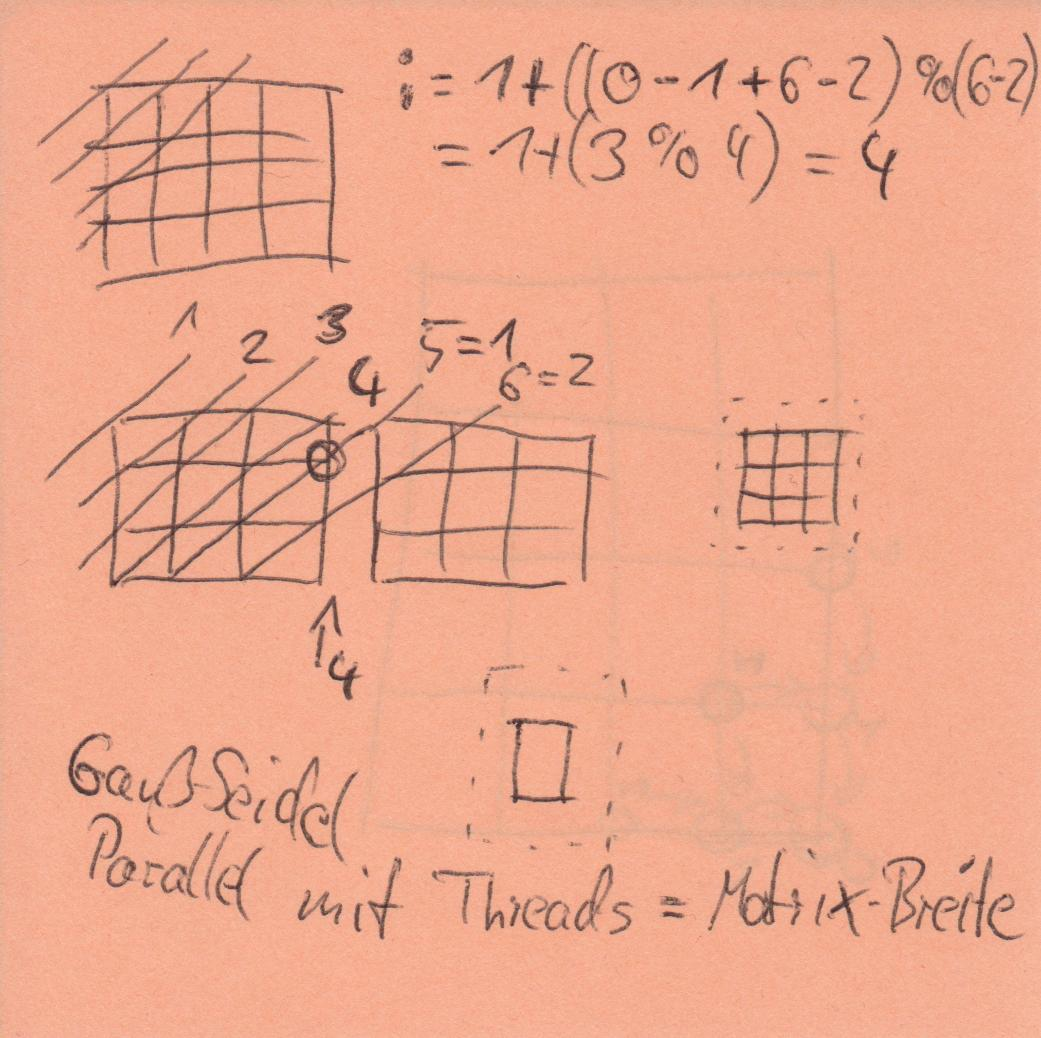
\includegraphics[width=0.5\textwidth]{gaussseidelskizze}
    \caption{Skizze zum Entwurfsgedanken zu Gauß"=Seidel, parallel.}
    \label{fig:gaussseidelskizze}
\end{figure}

Im Gegensatz zum Jakobi"=Verfahren sollte hier das GPU"=Potenzial geringer ausfallen.

\begin{quote}
    f) Ermitteln Sie den Speedup für verschiedene Problemgrößen für beide Verfahren (\(h = \frac{1}{2^l} \text{ mit } l = 1, 2, \dots, 6, \dots\)). Beurteilen Sie damit auch die Qualität ihrer Parallelisierungen.
\end{quote}

Joa, hier ist wohl noch was zu tun.

\end{document}
